% Generated from ICA_2.docx — re-run: python scripts/ica2_emit_latex.py
\chapter{Testing and Evaluation}
\label{ch:test}

\section{Introduction}

This chapter evaluates the IoT security monitoring application by assessing its functional correctness, reliability, and effectiveness in meeting the project objectives. Evaluation is conducted from both an objective perspective, through structured testing of system functionality, and a subjective perspective, through critical reflection on system behaviour, limitations, and overall success.

The testing strategy focuses on validating availability monitoring, anomaly detection, alerting behaviour, and security controls, as these represent the core contributions of the project. Given the academic nature of the artefact, testing is performed using a combination of manual functional testing, simulated failure scenarios, and observational analysis.

\section{Testing Strategy}

A black-box functional testing approach was adopted to evaluate system behaviour from the user's perspective, complemented by targeted white-box observations of backend behaviour through logs and database state. This approach was selected to reflect realistic usage scenarios while remaining appropriate for an undergraduate project context.

Testing was structured around the following key areas:

Device registration and management

Heartbeat submission and availability tracking

Detection of availability failures and anomalous behaviour

Alert generation and notification escalation

Security and access control mechanisms

System robustness under abnormal conditions

Rather than attempting exhaustive testing, the strategy prioritised critical paths that directly support the project's security-driven objectives.

\section{Functional Testing}

Device Registration and Management

Device registration functionality was tested by creating multiple IoT device entries through the authenticated API and dashboard interface. Tests confirmed that devices could be added, updated, and removed successfully, and that each device was uniquely identifiable within the system.

Device metadata, including device type, heartbeat interval, and alert preferences, was stored persistently and retrieved correctly. Invalid inputs, such as missing required fields or unsupported values, were rejected by the system, demonstrating effective input validation.

Outcome: Device management functionality behaved as expected and satisfied the functional requirements for device registration and configuration.

Heartbeat Monitoring and Availability Detection

Heartbeat functionality was tested by submitting periodic heartbeat messages for registered devices and observing changes in availability status. Devices that submitted heartbeats within the expected interval were correctly marked as online, with timestamps updated accordingly.

To simulate availability failures, heartbeat submissions were deliberately halted. After the configured tolerance threshold was exceeded, the system correctly flagged affected devices as offline or degraded. These state changes were recorded persistently and reflected accurately in the dashboard.

Outcome: Heartbeat monitoring reliably detected both normal operation and availability loss, supporting the project's central objective of availability-based security awareness.

Anomaly Detection Behaviour

Anomaly detection was evaluated by simulating abnormal conditions, including repeated missed heartbeats, sudden connectivity changes, and inconsistent reporting patterns. In isolation, minor irregularities did not immediately trigger high-severity alerts. However, when irregularities persisted or occurred in combination, the system generated alerts of increasing severity.

This behaviour demonstrated that the heuristic-based detection logic was capable of distinguishing between transient issues and more concerning patterns indicative of abnormal or potentially malicious activity.

Outcome: The anomaly detection logic functioned as intended, balancing sensitivity with resilience to false positives.

\section{Alerting and Notification Testing}

Alert generation was tested by triggering both availability failures and anomalous behaviour. Alerts were created with appropriate classifications and severity levels and were visible within the dashboard interface. Users were able to acknowledge and resolve alerts, supporting basic incident handling workflows.

Notification delivery was tested across supported channels where configuration was available. Severity-based escalation rules were observed to function correctly, with higher-severity alerts triggering more prominent notification methods. This validation ensures the system can escalate critical threats while actively mitigating alert fatigue for low-level anomalies (Hassan et al., 2020).

Outcome: Alerting and notification mechanisms provided timely and actionable feedback, reinforcing the system's role as a monitoring and awareness tool rather than a passive logging platform.

\section{Security and Access Control Evaluation}

Security controls were evaluated by attempting unauthorised access to protected endpoints and resources. API endpoints requiring authentication were inaccessible without valid credentials, and access to user-specific data was appropriately restricted.

Rate limiting and request validation mechanisms were observed to function as intended, reducing the risk of abuse or accidental overload in alignment with industry-standard API security practices (OWASP, 2024). API documentation interfaces were not publicly accessible and required authentication, limiting information exposure.

Outcome: The system demonstrated appropriate security controls for its intended scope and deployment context.

\section{Performance and Reliability Considerations}

Performance was evaluated qualitatively by observing system behaviour under repeated heartbeat submissions and concurrent user interactions. The asynchronous design enabled the system to process monitoring events without noticeable degradation in responsiveness.

Background monitoring tasks operated independently of user-facing requests, supporting continuous availability evaluation without blocking normal operation. Database indexing further contributed to acceptable query performance when retrieving device and alert data.

Outcome: While formal load testing was beyond the scope of the project, observed performance was consistent with the system's design goals and non-functional requirements.

\begin{figure}[htbp]
  \centering
  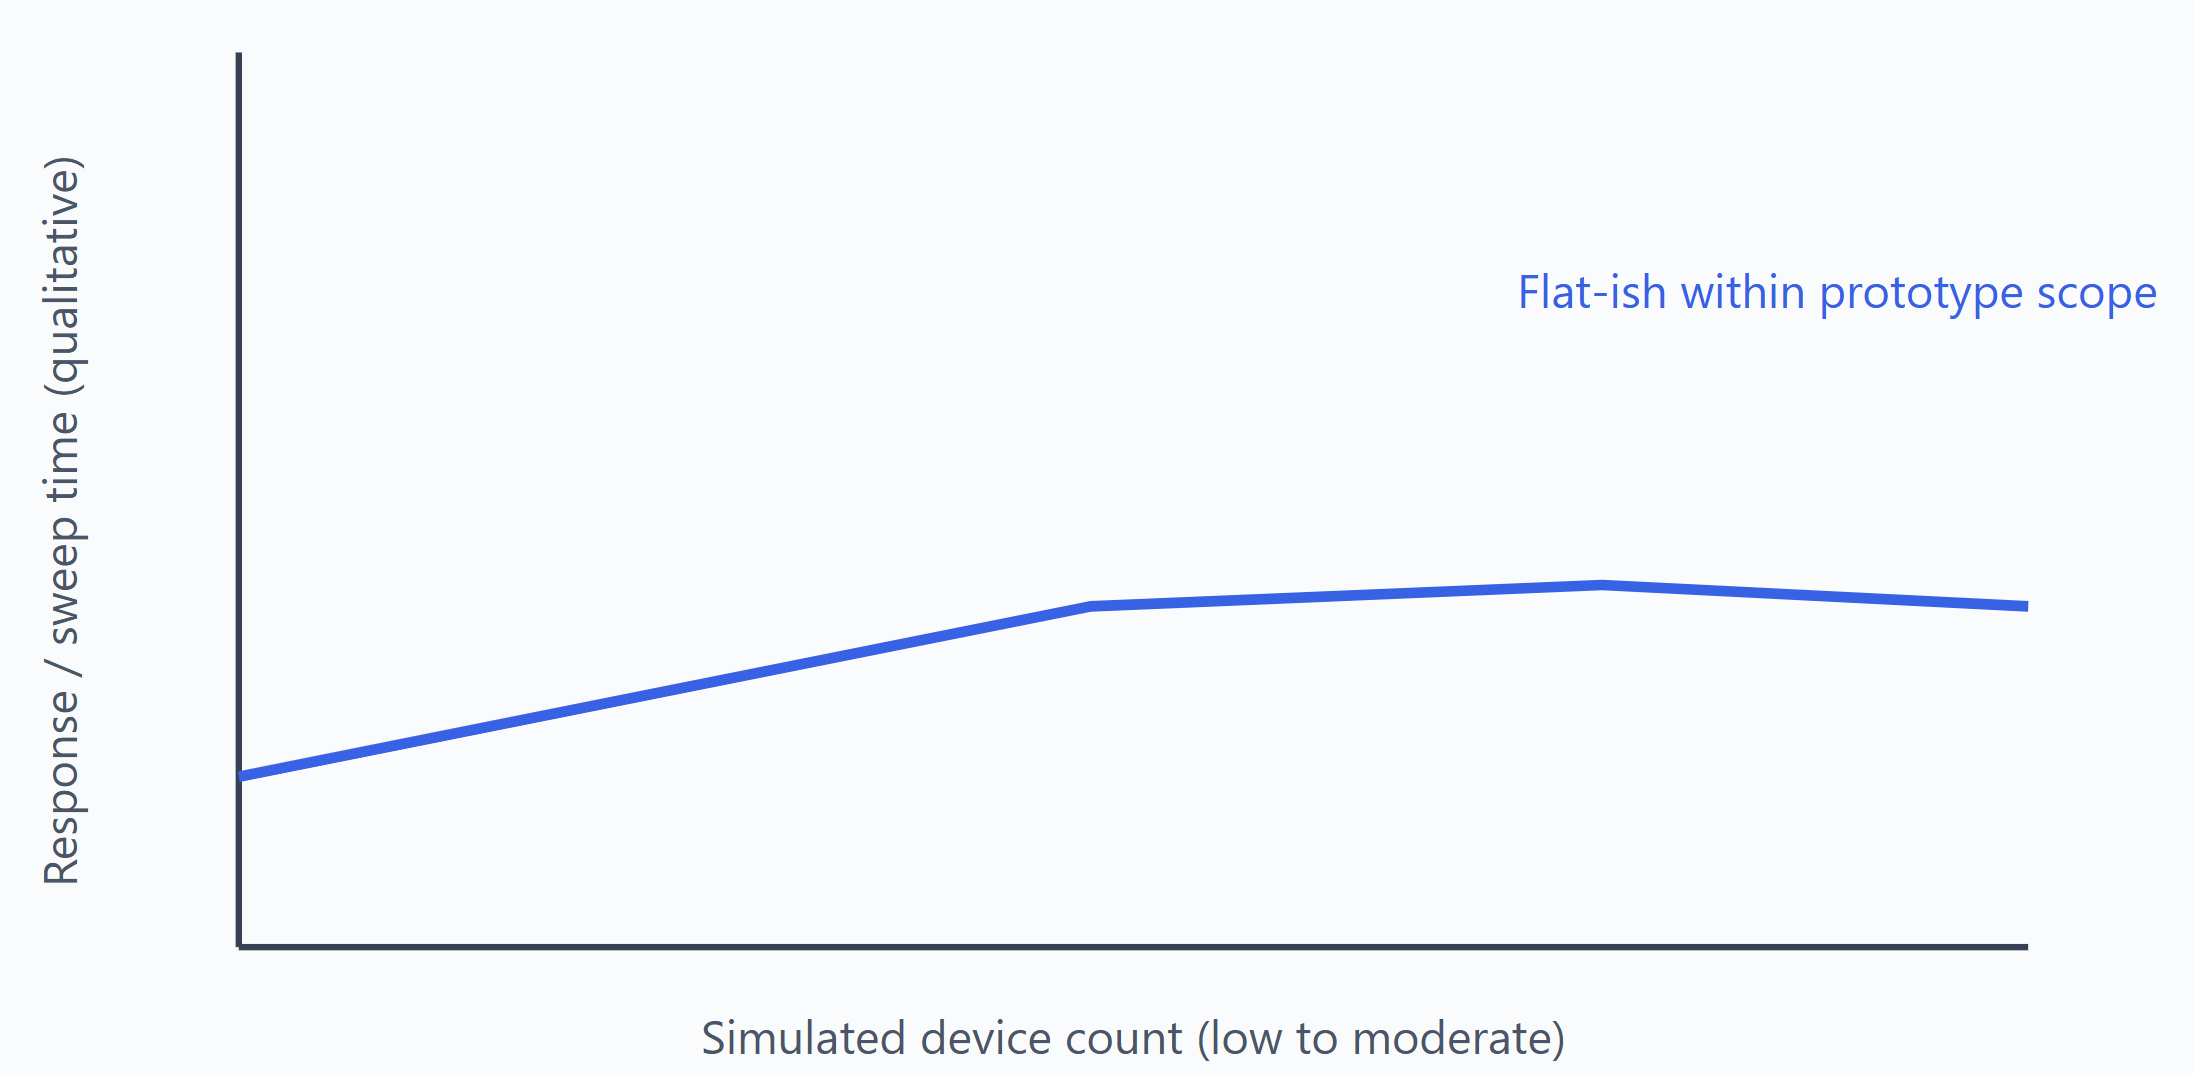
\includegraphics[width=0.92\textwidth]{figures/ICA2_embed_12.png}
  \caption{Qualitative Performance}
  \label{fig:ica2_12}
\end{figure}

\section{Limitations of Testing}

Several limitations affect the evaluation. Testing was conducted in a controlled environment with a limited number of simulated devices, which may not fully represent large-scale or highly dynamic deployments. Additionally, anomaly detection behaviour was evaluated qualitatively rather than through statistical analysis, reflecting the heuristic nature of the implementation when compared to machine-learning models (Ahmad \& Shah, 2024).

Notification testing depended on external services, which may behave differently under production constraints. These limitations are acknowledged and reflect the scope and constraints of an undergraduate project.

\section{Overall Evaluation of Project Success}

From an objective standpoint, the system successfully meets its core aims. It provides real-time visibility into IoT device availability, detects anomalous behaviour, and delivers timely alerts through configurable notification channels. The implementation demonstrates a coherent integration of security, availability monitoring, and usability considerations.

From a subjective perspective, the project represents a meaningful and practical response to a real-world problem. The focus on availability as a security concern, combined with lightweight monitoring techniques, results in a system that is accessible to non-expert users while still providing tangible security value.

\section{Summary}

This chapter has evaluated the IoT security monitoring application through structured testing and critical analysis. The results demonstrate that the system performs reliably within its intended scope and effectively addresses the problem identified earlier in the report. Identified limitations provide a basis for future improvement, which is explored in the following chapter.
